%%%%%%%%%%%%%%%%%%%%%%%%%%%%%%%%%%%%%%%%%%%%%%%%%%%%%%%%%%%%%%%%%
%
% Research background and fundamentals.
%
% author: Daniel Richter (d.richter@gsi.de)
%
% $Id: background.tex 2063 2012-07-25 18:01:51Z drichter $
%                                                              %%
%%%%%%%%%%%%%%%%%%%%%%%%%%%%%%%%%%%%%%%%%%%%%%%%%%%%%%%%%%%%%%%%%

\chapter{Research background and fundamentals}
\label{chap:background}
In this chapter the field of research will be introduced in which this
work is embedded and the conceptions required for the understanding of
the subsequent chapters will be clarified. The chapter consists of
four parts. The first section will introduce the physical, biological
and technical fundamentals of ion beam radiotherapy. Subsequently, the
problem of organ motion in radiotherapy will be addressed. In
particular, the implications for scanned ion beam therapy will be
emphasized. The necessary precautions for the deployment of scanned
ion beams in the presence of organ motion include a dedicated
treatment planning work flow which will be introduced in the third
section. Finally, a brief summary will be given.

\section{Ion beam therapy}

%
% dose conformity demonstration
%
\begin{figure}[p]
  \centering
  \includegraphics[width=0.7\textwidth]{imptvsimrt}
  \caption[Comparison of treatment plans for \acs{IMPT} and
  \acs{IMRT}]{Comparison of treatment plans for scanned carbon ions
    (\acl{IMPT}) with 2 fields (left) and x-rays (\acl{IMRT}) with 9
    fields (right). At a comparable level of dose conformity the dose to
    normal tissue is drastically reduced for the \ac{IMPT} plan. 
    Figure from \citep{Amaldi2005}. }
  \label{fig:background:imptvsimrt}
\end{figure}

%
% depth-dose profiles
%
\begin{figure}[p]
  \centering
  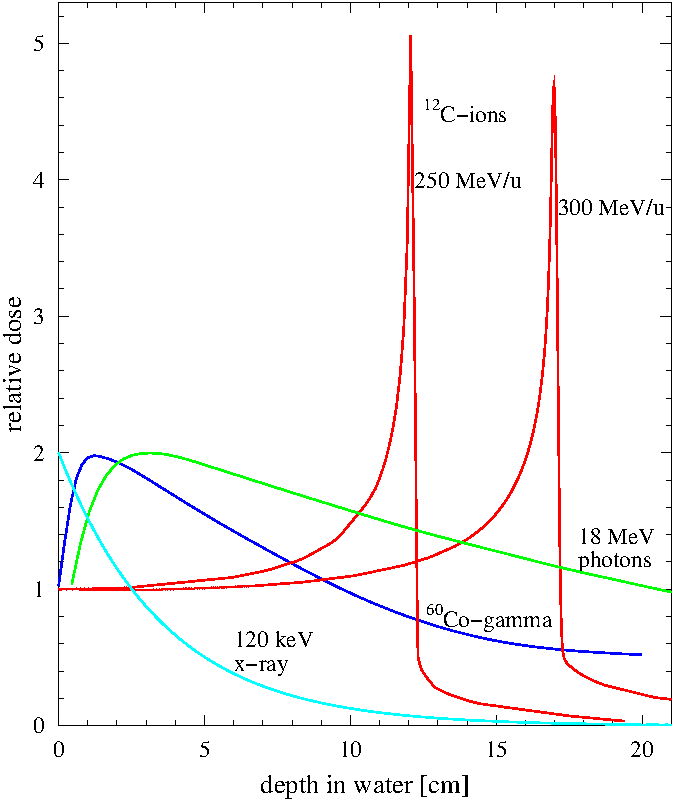
\includegraphics[width=0.6\textwidth]{depthdose}
  \caption[Depth-dose profiles for photons and \Ctw ions at different
  energies in water.]{Depth-dose profiles in water for photon and \Ctw
    ion radiation at different energies. The relative dose for \Ctw
    ions features a sharp maximum at the end of the finite range.  The
    photon curve drops exponentially after reaching a maximum in the
    entrance channel (build-up effect). The decrease of the Bragg
    maximum and the increased width is caused by a larger energy loss
    straggling. The tail after the Bragg maximum is caused by
    lighter fragments due to nuclear reactions. From
    \citet{Schardt2010}.}
  \label{fig:background:depthdose}
\end{figure}

In the past decades ion beam therapy has developed alongside
conventional x-ray therapy into a promising branch of radiation
therapy that offers superior dose distributions while sparing normal
tissue to a large extent (figure~\vref{fig:background:imptvsimrt}). In
1946 Robert\,R.\,Wilson first recognized the potential benefits of the
favorable depth-dose profile of ion beams for precision cancer therapy
\citep{Wilson1946}. Initial research on the physical and biological
properties of protons was followed by the first patient treatments
with proton beams at \ac{LBL}, Berkeley (\acs*{USA}) in the early
1950s \citep{Tobias1958}. The first proton therapy facility embedded
in a clinical environment started operation in 1990 at \ac{LLUMC}
(\acs*{USA}), soon followed by other facilities in the United
States, like the Francis\,H.\,Burr Proton Therapy Center at \ac{MGH}.

In the mid-1970s for the first time also heavier ions, mainly
He$^{2+}$ and \Netw, were employed for therapy at \ac{LBL},
to exploit their increased biological effectiveness. Shortly after the
end of the Berkeley ion therapy project in the early 1990s the heavy
ion therapy project at \ac{NIRS} in Chiba (Japan) started to employ
similar concepts for carbon ions like those pioneered at \ac{LBL}
\citep{Hirao1992}. Up to that time only passive beam delivery systems
had been used for ion beam therapy
(section~\ref{sec:background:passivedelivery}). In parallel, more
elaborate active beam delivery solutions
(section~\ref{sec:background:activedelivery}) were developed at
\ac{PSI}, Villigen (Switzerland) for protons \citep{Pedroni1995} and
at \ac{GSI}, Darmstadt (Germany) for \Ctw ions \citep{Haberer1993}.

From 1997--2008 the first patient treatments with a scanned heavy ion
beam were performed in a clinical trial at \ac{GSI} in close
collaboration with the \ac{DKFZ}, the \ac{UCHD} and the \ac{FZD}. Most
of the over 400 patients had tumors in the brain or at the base of the
skull. A dedicated treatment planning system was used for treatment
plan optimization, including full biological modeling of the enhanced
biological effectiveness of the \Ctw ions
\citep{Kraemer2000,Kraemer2000a}. Despite the technical complexity of
the system, the raster-scan technique has proven capable of
sub-millimeter accuracy and stable operation. Clinical follow-up
studies have shown high control rates for the treated tumor entities
combined with very low side effects \citep{Schulz-Ertner2007}. These
promising clinical results have encouraged the design and construction
of several dedicated heavy ion facilities based on the scanning
technique. As the first clinical center employing beam scanning, the
\ac{HIT} started clinical operation in 2009
\citep{Haberer2004,Combs2010}. A similar scanning system for carbon
therapy was implemented at \ac{NIRS} \citet{Furukawa2010a}. The first
centers using commercial beam scanning systems for protons were the
\ac{MDACC}, Houston (\acs{USA}) in 2006 and the \ac{RPTC}, Munich
(Germany) in 2009. Several other facilities are presently under
construction or in the planning phase. To date worldwide about 40
ion-beam therapy facilities are in operation, most of them using
proton beams with passive beam delivery systems. About 20 facilities
are in the design or construction phase, four of them are designed to
use carbon ion beams \citep{PTCOG2011}.

The following sections will introduce the physical, biological and
technical concepts of ion beam therapy. After a brief discussion of
the underlying physics of ion beams the implications for radiobiology
will be discussed. Since large parts of this work require a basic
understanding of the technical framework of ion beam delivery,
especially of the fully active scanner systems as they are used at
\ac{GSI} and \ac{HIT}, a separate section will be dedicated to their
introduction.

% references for MGH, Loma Linda\\
% a few more details on GSI pilot project, esp. clinically?\\
% mention CNAO?\\

% how many patients
% clinical motivation

\subsection{Physical properties}
The main rationale for using ion beams for localized tumor therapy is
their favorable depth-dose profile compared to photons. A comparison
of the depth-dose curves for photons and ions with different energies
is shown in figure \vref{fig:background:depthdose}
\citep{Schardt2010}. After a shallow maximum in the entrance region,
caused by the dose build-up due to forward scattered Compton electrons
\citep{Alpen1998}, the photon depth dose profile drops exponentially
with the penetration depth. In contrast, the ion depth dose-curve
features a distinct narrow peak with a sharp dose fall-off at the end
of the particle range. This curve is called \emph{Bragg curve} or
\emph{Bragg peak}, named after its discoverer, Sir William Henri Bragg
\citep{Bragg1905}. The position of the Bragg peak in depth can be
precisely controlled by varying the kinetic energy of the incident
ions. This 'inverse' depth-dose profile, the small lateral scattering
and the finite particle range evidently are particularly appealing for
the treatment of deep-seated tumors, sparing normal tissue, especially
behind the Bragg peak. The underlying physics will be discussed in the
following sections.

\subsubsection{Dose deposition and electronic stopping}
%
% dE/dx plot
%
\begin{figure}[tpb]
  \centering
  \includegraphics[width=0.7\textwidth]{energyloss_c12_p}
  \caption[Specific energy loss of \Ctw and protons in water.]{
    Specific energy loss of \Ctw and protons in water
    \citep{Schardt2010}.}
  \label{fig:background:energyloss}
\end{figure}

The dose, $D$, deposited in the tissue is of central importance in
radiotherapy and is defined by the ratio of the absorbed energy $\dE$
per mass element $\dd m$ \citep{ICRU51}:
\begin{equation}
  D= \frac{\dE}{\dd m}\quad\left[\SI{1}{\gray}=\SI[per-mode=symbol]{1}{\joule\per\kilogram}\right].
  \label{eq:background:physdose}
\end{equation}
For a parallel beam traversing a thin layer of material the absorbed
dose is determined by the \emph{specific energy loss} per unit length
or \emph{stopping power} of the particles, \dEdxt, the fluence, $F$, and
the material mass density, $\rho$:
\begin{equation}
  D[\si{\gray}]=\num{1.6e-9}\times
  \dEdxm\left[\si{\kilo\electronvolt\per\micro\meter}\right]\times
  F\left[\si[per-mode=reciprocal]{\per\square\centi\meter}\right]\times
  \frac{1}{\rho}\left[\si{\cubic\centi\meter\per\gram}\right].
  \label{eq:background:fluencedose}
\end{equation}
Different energy loss processes contribute to the total stopping
power, \dEdxt. The required maximum penetration depth of about
\SI{30}{\centi\meter} in the human body corresponds to kinetic
energies of protons and carbon ions of
\SIlist{200;430}{\mega\electronvolt\per\atomicmassunit},
respectively. In this medium relativistic regime the total stopping
power is dominated by inelastic scattering of the ions with the target
electrons. The collisions result in ionization and excitation of the
target atoms. Elastic collisions with the target nuclei (nuclear
stopping) only contribute significantly to the total energy loss at
very small particle energies, \ie near the end of their
range. Radiative energy losses play a role in the highly relativistic
regime only and therefore can be neglected as well
\citep{Nakamura2010}. Thus, the considerations will be limited to the
electronic stopping power here.
% The reader is referred to \citet{Nakamura2010} for a detailed review
% of other interaction processes of charged particles with matter.

In the energy range of interest the electronic stopping power is well
described by the Bethe formula
\citep{Bethe1930,Bloch1933,Bloch1933a,Fano1963}
\begin{equation}
  \dEdxmbr=\frac{4\pi
    e^4Zz^2}{m_ec^2\beta^2}\left[\ln{\left(\frac{2m_ec^2\beta^2}{I(1-\beta^2)}\right)}
    -\beta^2-\frac{C}{Z}\right]
  \label{eq:background:bethe}
\end{equation}
Here $\beta=v/c$ is given by the velocity $v$ of the incident particle
normalized to the speed of light $c$. $Z$ and $z$ are the nuclear
charges of the target and the projectile, respectively. $m_e$ denotes
the mass and $e$ the elementary charge of the electron. The mean
ionization potential, $I$, of the target atoms or molecules is usually
obtained empirically and is around \num{75}--\SI{78}{\electronvolt}
for liquid water \citep{Schardt2008,Paul2007,Kumazaki2007}. Values for
other materials are summarized in \citet{ICRU49,ICRU37}. Equation
\eqref{eq:background:bethe} also includes the shell correction term,
$C/Z$, which takes into account the orbital velocities of the target
electrons at low particle energies.
% The density correction term, $\delta/2$, considers material
% polarization effects at highly relativistic energies.
Detailed reviews on the shell correction term and other low energy
corrections of the electronic stopping power are given in
\citep{ICRU49,Ziegler1999}.

Figure~\ref{fig:background:energyloss} shows the mean electronic
stopping power for carbon ions and protons in the relevant energy
regime for ion beam therapy \citep{Schardt2010}. The energy loss
increases sharply with decreasing particle velocity, due to the
$1/\beta^2$ dependence in \eqref{eq:background:bethe}. At lower
velocities recombination processes with the target electrons gradually
lower the effective charge of the projectile and result into a
decreasing energy loss rate after reaching a maximum at a specific
energy of $\approx$\SI{350}{\kilo\electronvolt\per\atomicmassunit} in
the case of \Ctw ions. This effect can be incorporated into
\eqref{eq:background:bethe} by replacing $z$ with the effective
charge $z_\text{eff}$. Empirically $z_\text{eff}$ can be parametrized
using Barkas' formula \citep{Barkas1964}:
\begin{equation}
  z_\text{eff}=z\left[1-\exp(-125\beta z^{-2/3})\right].
\end{equation}
Figure~\ref{fig:background:energyloss} also shows the minor
contribution of the elastic scattering with the target nuclei at the
very end of the particle range (dashed line).

%
% lateral range
%
% \begin{figure}[tpb]
%   \centering
%   \includegraphics[width=0.7\textwidth]{ion_ranges}
%   \caption[Mean range for different ion species in water.]{
%     Mean range for different ion species in water \citep{Schardt2010}.}
%   \label{fig:background:ionrange}
% \end{figure}

\subsubsection{Range straggling and lateral scattering}
The Bethe formula describes the \emph{mean} electronic stopping power
only. However, energy loss by inelastic Coulomb scattering is governed
by large statistical fluctuations. For a beam of many slowing down
particles this results in a significant broadening and a reduced
peak-to-entrance dose ratio of the Bragg peak
(figure~\ref{fig:background:depthdose}). In the limit of a large
number of collisions or thick layers the energy loss obeys a Gaussian
probability distribution. The energy loss fluctuations directly
translate into \emph{range straggling} \citep{Bohr1940,Ahlen1980}. The
ratio $\sigma_R/R$ of the straggling width $\sigma_R$ and the mean
range $R$ is proportional to $1/\sqrt{M}$ with $M$, the ion
mass. Thus, the broadening of the Bragg peak is less pronounced for
heavier ions. For example the ratio $\sigma_R/R$ is about a factor 3.5
smaller for \Ctw ions than for protons \citep{Schardt2010}.

% 
% this in?
%
% For practical reasons, however, a deliberate broadening of the Bragg peak
% by passive devices inserted into the beam line can be even desirable
% in the case of slice-by-slice scanning systems to reduce the treatment
% time (section \ref{sec:background:beamdelivery}).

On their way through the material the particles undergo small lateral
deflections, due to elastic scattering off the target nuclei. This has
been described analytically by \citet{Moliere1948} and is in very good
agreement with measurements \citep{Gottschalk1993}. Heavier target
nuclei cause a larger angular spread for the same thickness of a
material layer. The angular spread also depends significantly on the
particle's energy and increases towards the lower end of the particle
range. Compared to a proton beam with the same range in water of about
\SI{16}{\centi\meter} the angular spread of a \Ctw beam is more than
three times smaller \citep{Schardt2010}. In clinical practice ion
beams therefore offer significantly sharper dose gradients and better
sparing of normal tissue \citep{Weber2009}.
% A more detailed comparison of the lateral
%scattering behaviour of protons and \Ctw ions was given by


\subsubsection{Nuclear fragmentation}
%
% abrasion ablation
%
%\begin{figure}[tpb]
%  \centering
%  \includegraphics[width=0.7\textwidth]{fragmentation}
%  \caption[Nuclear fragmentation.]{
%    Nuclear fragmentation \citep{Schardt2010}.}
%  \label{fig:background:fragmentation}
%\end{figure}


The cross section for nuclear interactions is orders of magnitude
smaller than for Coulomb interaction. Nuclear fragmentation reactions
nevertheless play a significant role at large penetration depths. For
ions heavier than protons projectile fragments contribute
significantly to the absorbed dose and lead to dose tails at the
distal end of the depth dose profile
(figure~\ref{fig:background:depthdose}). To a lesser extent
fragments of the target nuclei also contribute. However, these have
very low ranges and do not travel with the beam. For all ions except
protons projectile fragmentation is the dominant process. In
collisions of the projectile with a target nucleus a partial
disintegration of the projectile results into excited states of the
remaining projectile fragments, followed by de-excitation through the
emission of nucleons, nucleon clusters and photons. Detailed reviews
of the underlying fundamental processes have been published elsewhere
\citep{Goldhaber1978,Huefner1985,Lynch1987}.

Nuclear fragmentation leads to a loss of primary particles and a
build-up of mostly lower-$Z$ fragments increasing with depth. For
kinematical reasons these lighter fragments move with approximately
the same velocity and into the same direction as the primary
particles. While the rare heavier fragments are stopped rather
quickly, the lighter hydrogen and helium fragments have larger ranges
and produce significant dose tails behind the Bragg peak. Due to the
exponential loss of primary particles, the depth dose profiles feature
a gradually diminishing peak-to-entrance dose ratio (figure
\ref{fig:background:depthdose}). Additionally the profiles are
increasingly broadened by straggling \citep{Schardt2010}. These
effects are more pronounced for heavier ions and become intolerable
for therapy for ions heavier than \Netw \citep{Kraft2000}. Taking into
account the dose contributions of nuclear fragments based on measured
data is essential for treatment planning. This is particularly
important for the inclusion of the biological efficacy of the
different constituents of a mixed particle beam (section
\ref{sec:background:radiobiology}). For this reason, measurements have
been performed at many centers to assess the magnitude of
fragmentation, the relative composition of isotopes and their
contribution to the absorbed dose
\citep{Maccabee1974,Schimmerling1983,Llacer1984,Schall1996,Haettner2006}.


\subsubsection{Track structure and radial dose distribution}
%
% track structure
%
\begin{figure}[p]
  \centering
  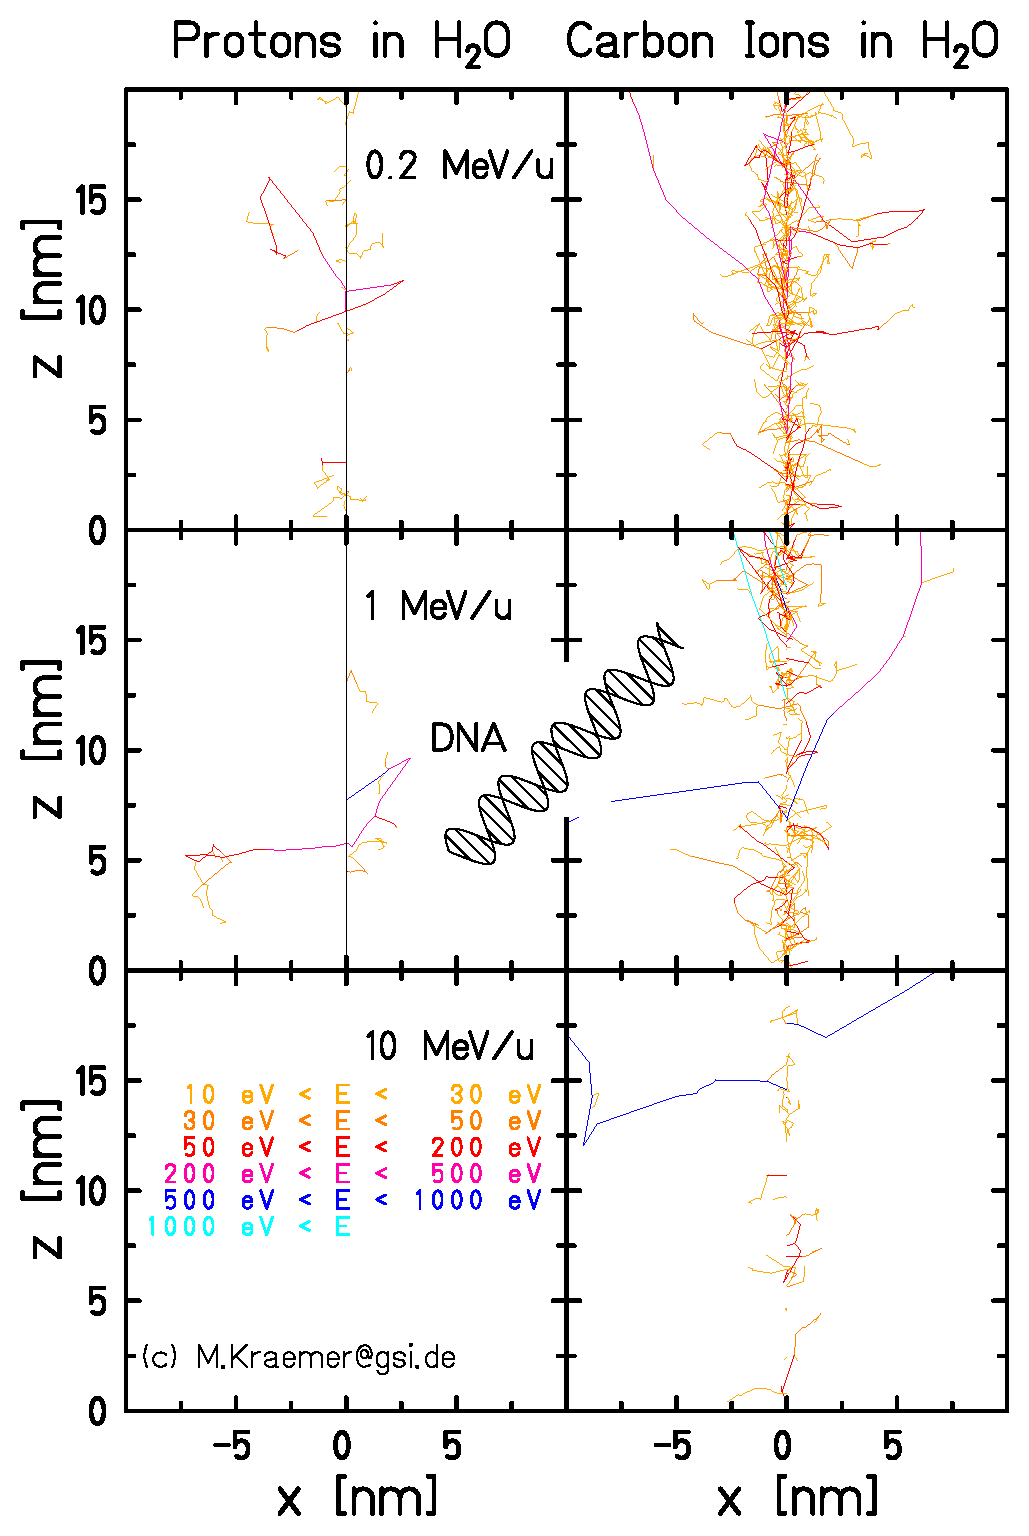
\includegraphics[width=0.8\textwidth]{trackstructure}
  \caption[Simulated secondary electron paths created by protons and
  carbon ions at different energies.]{ Simulated paths of secondary
    electrons with different energies created by protons and carbon
    ions at different specific energies. The \acs{DNA} molecule 
    illustrates the geometrical dimension of the track structure.
    Figure courtesy of M.\,Kr\"amer.}
  \label{fig:background:trackstructure}
\end{figure}
Ions lose their energy by ionization and excitation of the target
electrons via inelastic Coulomb scattering. The liberated electrons
undergo frequent elastic and inelastic scattering and may cause
secondary ionization of the target atoms if their kinetic energy is
sufficiently high. For electron energies larger than
$\approx$\SI{50}{\electronvolt} ionization is the dominant process
leading to large numbers of additional electrons
\citep{Kraft2000,Schardt2010}. The energy spectrum of the electrons
defines both, the radial dose profile around the track and the track
diameter. Since most of the electrons only receive small energy
transfers or are scattered in forward direction, the radial dose is
concentrated at the track core and quickly falls off with larger
radial distances~$r$. The existing models
\citep{Chatterjee1976,Katz1999} and Monte Carlo codes
\citep{Paretzke1986,Kraemer1995} all predict an approximate $1/r^2$
dependence for the radial dose fall-off. This has been confirmed by
dosimetry experiments \citep{Varma1977}. For the dose contribution at
smaller radii than \SI{10}{\nano\meter} a flat profile is often
assumed \citep{Scholz1996}. The maximum track extension,
$r_\text{max}$, is determined by the energy of the most energetic
electrons and empirically can be related to the energy, $E$, of the
primary particle: $r_\text{max}\propto E^{1.7}$
\citep{Kiefer1986}. Due to the $z^2$ and the $1/\beta^2$ dependence of
equation \eqref{eq:background:bethe}, the track structure of ions is
considerably dependent on the ion species and energy. Figure
\vref{fig:background:trackstructure} demonstrates the much more
dense ionization patterns of carbon ions compared to protons at
different energies obtained by a Monte Carlo simulation
\citep{Kraemer2010}. Most of the electrons have very low energies,
resulting into ranges on the nanometer scale and a very localized
energy deposition. For decreasing energy the increasing stopping power
of the ions translates into significantly larger numbers of secondary
electrons. The energy deposition of the electrons in the material is
often described using the \emph{\ac{LET}} or \emph{restricted energy
  loss}. The \ac{LET} is closely related to \dEdxt and defines the
\emph{locally} transferred energy to the medium, excluding
contributions of electrons with energies above a certain threshold
\citep{ICRU37,Nakamura2010}.


\subsection{Radiobiology}
\label{sec:background:radiobiology}


% figure 4DCT
%
\begin{figure}[tbp]
  \centering
  \includegraphics[width=0.8\textwidth]{radiationdamage}
  \caption[Direct and indirect radiation damage to the \ac{DNA}.] {
    (a) Direct and indirect radiation damage to the \ac{DNA}. Direct
    damage is caused by energy deposition in direct hits from
    electrons liberated in ionization processes. Free hydroxyl
    radicals (OH), formed by ionization in the hydrolysis of water,
    can cause indirect damage to the \ac{DNA} in chemical
    reactions. (b) Schematic illustration of selected types of
    radiation damage to the \ac{DNA}. The effectiveness of the repair
    mechanisms of cells depends on the complexity of the damage. }
  \label{fig:background:radiatdamage}
\end{figure}
The goal of radiotherapy is to inactivate all tumor cells and thus
prevent further cell growth and cell division. Radiation damage can be
induced everywhere in the cell. However, it is commonly acknowledged
that the most critical structure of a cell with respect to radiation
damage is the \acf{DNA} which is located inside the cell nucleus
\citep{Munro1970}. Although cells have a number of sophisticated
repair mechanisms, the repair capacities are limited, depending on the
type of damage \citep{Sancar2004}. Commonly, direct and indirect
radiation-provoked effects are distinguished, as shown schematically
in figure~\ref{fig:background:radiatdamage}a. \textbf{Direct effects}
are caused by the ionization of a \ac{DNA} constituent
itself. Consequently, molecular bonds can be destroyed and result in
break-up of a single or both \ac{DNA} strands
(figure~\ref{fig:background:radiatdamage}b).  Furthermore, randomly
created new bonds may be formed and alter the \ac{DNA}
structure. While single-strand breaks can be repaired rather
efficiently, double-strand breaks often result in eventual cell
death. In general, they are considered the critical events for lethal
lesions. Direct effects are of increased importance for ion
radiation. For more sparsely ionizing radiation like photons, however,
the majority of the radiation-induced effects are \textbf{indirect
  effects}. Most notably, free and highly reactive hydroxyl-radicals
(OH) are created in the radiation-induced hydrolysis of water
molecules surrounding the cell nucleus. Although they have a short
lifetime, they can migrate over several nanometers and are capable of
damaging the \ac{DNA} structure. Due to larger recombination of
radicals these effects are of less importance for ion radiation.
Direct and indirect radiation damage occur in parallel and can
accumulate to an extent so that the repair of the \ac{DNA} is no
longer possible.
 
A key advantage of heavy ion beams in radiotherapy applications is
their increased biological efficiency in the target region, compared
to photon irradiation. The large ionization densities along the ion
tracks at the Bragg peak can cause clustered lesions of the \ac{DNA}
molecule, \ie multiple double-strand breaks, which have a small
probability of being repaired, resulting into subsequent cell
death. Figure \ref{fig:background:trackstructure} illustrates the
spatial distribution of the secondary electron halo around the track
of protons and \Ctw ions in relation to the size of a \ac{DNA}
molecule. Most of the insight into the response of cells to radiation
has been acquired for photon radiation. Hence, the biological effect
of ion radiation is commonly described relative to a reference photon
response, using the concept of the \emph{\ac{RBE}}. The \ac{RBE} is
defined as the ratio of the reference photon dose to the dose level
needed for a specific ion radiation in order to achieve the same
biological effect (isoeffect)
\begin{equation}
  \text{RBE}=\frac{D_\gamma^\text{ref}}{D_\text{ion}}\,\,\bigg|_\text{isoeffect}\,.
  \label{eq:background:rbe}
\end{equation}
Comparisons of \acs{RBE} values are valid only for the same effect and
effect level (biological endpoint) and the same reference
radiation. In ion beam tumor therapy the most relevant biological
endpoints are cell survival and certain normal tissue side effects. In
the following the term \ac{RBE} is used synonymously with the \ac{RBE}
for cell survival. Figure \vref{fig:background:dosedependence}
illustrates the calculation of \ac{RBE} at the \SI{10}{\%} and
\SI{1}{\%} survival level.  The survival curve for ion irradiation
shows a steeper fall-off in survival while the x-ray curve exhibits a
characteristic shoulder. Consequently, the \ac{RBE} values are
dependent on the dose level.  In addition to the physically absorbed
dose, as defined in equation \eqref{eq:background:physdose}, the term
of a \emph{photon-equivalent} or \emph{biological dose} incorporating
the \ac{RBE} is often convenient. The difference to the \emph{physical
  dose} is marked by expressing the biological dose in units of
\si{\GyE} or \si{\GyRBE}. The latter notation is recommended by the
\ac{ICRU} and will be used in the following \citep{ICRU78}.  The
shouldered curve describing the cell survival, $S$, in dependence of
the dose level, $D$, is commonly described by an exponential
linear-quadratic model (LQ-model) \citep{Fowler1989}:
\begin{equation}
  S(D)=\exp\left(-\alpha D-\beta D^2\right)\quad.
\end{equation}
The ratio $\alpha/\beta$ is characteristic of the tissue type and
radiation quality and is related to the repair capacities of the
cells. A large $\alpha/\beta$ ratio indicates a small repair capacity
or, equivalently, a large radiation sensitivity.


\begin{figure}[tbp]
  \centering
  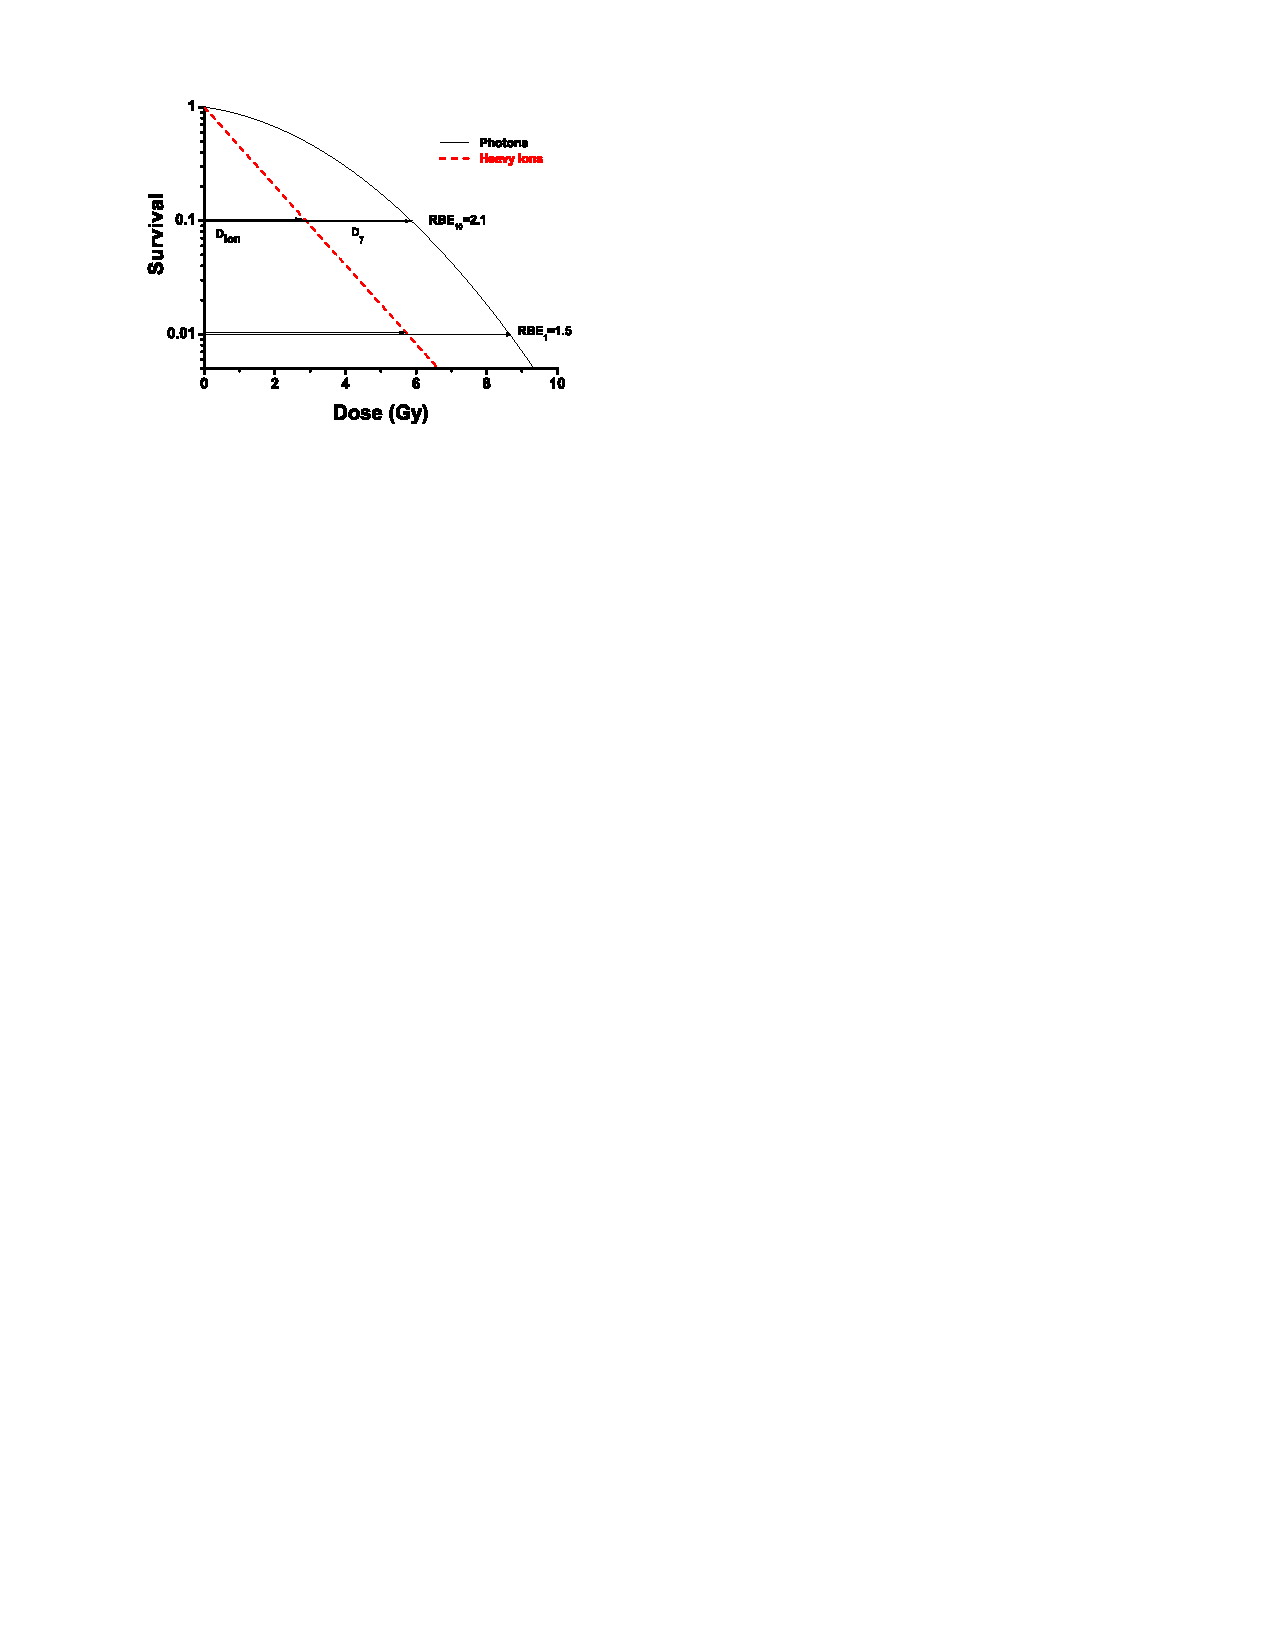
\includegraphics[width=0.6\textwidth]{dose_dependence}
  \caption[Dose dependence.]{Sketch of typical cell survival curves
    for photon and heavy ion irradiation. The ion curve shows a
    steeper decrease with dose and lacks the characteristic shouldered
    form of the photon curve. The \ac{RBE} value depends on the
    survival level, or equivalently, on the dose level
    \citep{Schardt2010}.}
  \label{fig:background:dosedependence}
\end{figure}

% LQ model, TCP and NTCP?

The systematics of the \ac{RBE} are complex. Apart from the biological
endpoint the \ac{RBE} depends on other physical and biological
parameters, the most important ones being the dose level, the
\ac{LET}, the particle species and the tissue type. The reader is
referred to the reviews by \citet{Kraft2000}, \citet{Scholz2003},
\citet{Fokas2009} and \citet{Schardt2010} for detailed discussion of
the various \ac{RBE} systematics.
%
% probably too much here
% 
% of which the most important ones shall be summarized here
% in brief.
% \begin{description}
% \item[dose level:] Figure \ref{fig:background:dosedependence} shows
%   a sketch of a typical configuration of survival curves observed
%   experimentally for photons and carbon ions. Survival curves for
%   photons often exhibit a shoulder while heavy ions have a purely
%   exponential form. Depending on the survival level the ratio of
%   $D\gamma$ and $D_\text{ion}$ results in different \ac{RBE}
%   values. In the figure this is illustrated for the \SI{10}{\%} and
%   \SI{1}{\%} survival level.
% \item[linear energy transfer:] The \emph{\ac{LET}} or \emph{restricted
%     energy loss} is closely related to \dEdxt defining the
%   \emph{local} energy tranferred to the medium
%   \citep{ICRU37,Nakamura2010}.  With increasing \ac{LET} the
%   propability for cell survival is more and more reduced. At an
%   \ac{LET} in the range of
%   $\approx$100--\SI{200}{\kilo\electronvolt\per\micro\meter} the
%   locally deposited dose most efficiently reduces the probability for
%   cell survival leading to a maximum in \ac{RBE}. At even higher
%   \ac{LET} the additional dose can have no additional effect on cell
%   survival, since the dose deposited in a single particle traversal is
%   already sufficient to kill the cell. The \ac{RBE} therefore is
%   diminished for further increased \ac{LET}. This is known as the
%   \emph{overkill effect}.
% \item[particle species:] Heavier ions feature their \ac{RBE} maximum
%   at higher \ac{LET} values than lighter particles. At the same
%   \ac{LET} value heavier ions are much faster than lighter ions and
%   have larger track radii with less ionisation density. Consequently
%   their \ac{RBE} maximum is reached for correspondingly smaller
%   velocities at higher \ac{LET}. In figure
%   \vref{fig:background:letdependence} the \ac{LET} dependence of the
%   \ac{RBE} is shown for different ion species. The data from
%   \citet{Belli1998} and \citet{Furusawa2000} show the characteristic
%   \ac{LET} dependence with peaks at particle-dependent values of
%   \ac{LET}.
% \item[tissue type:] The \ac{RBE} depends on the radiosensitivity of
%   the respective tissue which is related to the repair capacity of the
%   cells. In general it has been found experimentally that tissues with
%   large repair capacities show lower \ac{RBE} maxima than more
%   radiosensitive tissues.
% \end{description}
%
% \begin{figure}[tbp]
%   \centering
%   \includegraphics[width=0.7\textwidth]{let_dependence}
%   \caption[LET dependence.]{LET dependence of the \ac{RBE} for
%     protons, He and Ne ions. The position of the \ac{RBE} maximum
%     is shifted to larger \ac{LET} values for heavier ions. Experimental data from
%     \citet{Belli1998} and \citet{Furusawa2000}. Figure from
%     \citep{Scholz2003}.}
%   \label{fig:background:letdependence}
% \end{figure}
It should be noted that the increased biological effectiveness of ions
can only be exploited to the maximum extent if it is more pronounced
in the tumor than in the normal tissue. Due to the \ac{LET} dependence
the \ac{RBE} is elevated also in the entrance channel for relatively
heavy ions, like argon.  In contrast, carbon ions feature a sharp
\ac{RBE} maximum which coincides with the Bragg peak
\citep{Kraft2000}. In proton therapy the assumption of a constant \ac{RBE}
of 1.1 over the treatment field is feasible \citep{Paganetti2002}. For
carbon ions the \ac{RBE} varies over a factor of ten from values close
to 1.0 in the entrance channel to typical values around 5.0 in the
target region. Even higher values of around 10.0 can result in the normal
tissue beyond the field edges \citep{Kraft2009}. 

The large variations in \ac{RBE} facilitate the need for a biological
model which is able to predict the \ac{RBE} in a mixed radiation field
over a wide range of atomic numbers and energies. At \ac{GSI} this is
done using the \emph{\ac{LEM}} developed by Scholz \etal
\citep{Scholz1994,Scholz1996}.  The model predicts the biological
efficacy starting from the dose dependence of the cell inactivation by
x-rays which was measured in cell experiments, the radial dose
distribution around the particle track and the size of the cell
nucleus. The general underlying assumption is that there is no
fundamental difference in the physical dose deposited by photons or
ions via secondary electrons. The different biological response
solely originates from the characteristics of the dose deposition
pattern. While for photons a homogeneous dose distribution over the
cell nucleus can be assumed, particle irradiation leads to highly
localized dose distributions at the same total dose. Assuming the
x-ray response is valid also for these high local doses, the dose
response for ions can then be determined according to the x-ray
response at the same dose level. Improved versions of the \ac{LEM}
have been published over the years
\citep{Elsaesser2006,Elsaesser2007,Elsaesser2009} and the model has
been successfully tested in numerous cell experiments
\citep{Mitaroff1998,Kraemer2000a,Kraemer2003} and is incorporated into
the \ac{GSI} treatment planning system which has been used in the past
in clinical routine in the \ac{GSI} pilot project from 1995--2008
\citep{Kraemer2000,Kraemer2000a} as well as at \ac{HIT} since 2009.


\subsection{Beam delivery}
\label{sec:background:beamdelivery}
Ion beam therapy requires complex beam delivery systems capable of
accelerating ions to therapeutic energies of several hundred
\si{\mega\electronvolt\per\atomicmassunit}, transporting the ion beams
to the treatment area and guiding them onto the target with the
necessary accuracy.  Particle acceleration is typically realized using
either cyclotron or synchrotron accelerators. \textbf{Cyclotrons}
nowadays can be built very compact and offer continuous beams with
stable beam intensities.  However, active energy variation is not
possible with this design, therefore passive degraders have to be used
at the cost of beam intensity and quality. \textbf{Synchrotrons} in
contrast provide pulse-to-pulse active energy variation. The beams
have to be injected into the synchrotron ring by a dedicated linear
accelerator. Ion optics are used to keep the ions on track during
further acceleration and storage. % The pulsed beam structure has
% implications for modern treatment modalities like gating (section
% \ref{sec:background:mitigation}) as beam availability has a time
% structure. Also the intensity structure of the pulses (spills) is of
% interest. So-called \emph{knock-out} extraction has been developed
% by \citep{Noda1996} allowing for very controllable beam extraction.
While cyclotrons are used in most proton facilities, to date all heavy
ion centers employ the synchrotron solution.

A single Bragg peak does not adequately cover the target volume with a
homogeneous dose, consequently the beams need to be shaped, once the
beam has been guided to the treatment area. Two different strategies
have been developed over the years and are in use today in different
variations. The following section will introduce passive and active
beam shaping systems, concentrating on the fully active beam delivery
system at \ac{GSI} and \ac{HIT} which are of major interest in this
work.

\subsubsection{Passive beam shaping}
\label{sec:background:passivedelivery}
%
% passive beam delivery
%
\begin{figure}[tbp]
  \centering
  \includegraphics[width=0.75\textwidth]{passivedelivery}
  \caption[Schematic of a passive beam delivery system.]{Schematic of
    a passive beam delivery system. The narrow, mono-energetic beam is
    scattered to match the required lateral dimensions. Lateral and
    longitudinal adaption to the tumor is performed by different
    passive modulator devices. The distal edge of the tumor is
    conformed by an individually machined compensator. The hatched
    area indicates the resulting inevitable irradiation of normal
    tissue. Figure redrawn from \citep{Schardt2010}.}
  \label{fig:background:passive}
\end{figure}
Passive beam shaping systems employ different devices inserted into
the beam line to manipulate the beam laterally and longitudinally. In
the following, the basic concept shall be presented. More detailed
overviews of passive beam shaping techniques and the specific devices
can be found in \citet{Chu1993, Kraft2000} and
\citet{Gottschalk2008}. In figure~\ref{fig:background:passive} the
concept of passive beam shaping is shown schematically. First the
initial narrow beam is broadened with a scattering device to generate
a broad and flat lateral beam profile. Here, \eg, passive double
scattering systems or magnetic wobbler devices are frequently used
\citep{Kraft2000}. The mono energetic beam beam is then spread out
over the required depth using a range modulator. In practice, ridge
filters or rotating wheels of varying thickness are employed
\citep{Chu1993}.  Stacking of Bragg peaks at different depths results
into a so-called \emph{\ac{SOBP}}. The \ac{SOBP} is then shifted to
the needed depth using a range shifter. Again, this is a passive
absorber that is chosen at the required material thickness. The
discussed devices are not patient-specific although, \eg, a whole
library of range modulators may be needed for different longitudinal
field extensions. In addition, devices machined individually for each
patient are needed to tailor the beam to the respective target as much
as possible.  The lateral extension of the treatment field is defined
by a collimator, typically made from brass, in order to yield sharp
lateral field gradients.  The collimator is followed by a range
compensator usually made from \ac{PMMA} and designed such that the
\ac{SOBP} is adjusted to the distal edge of the tumor in \ac{BEV}. A
major deficiency of the compensator is the incapacity to form the
proximal edge of the tumor. This results into parts of the \ac{SOBP}
dose being deposited in surrounding normal tissue, as depicted by the
hatched area in figure~\ref{fig:background:passive}.

For historical reasons, the vast majority of ion beam therapy
centers worldwide employ passive beam delivery techniques.  Although
passive beam delivery techniques have been refined over the years,
they carry intrinsic limitations, \eg, a restricted tumor
conformity, the need for patient-specific hardware and an
inflexibility in dose modulation.  Many of the limitations can be
overcome using active beam shaping techniques which will be introduced
in the next section.

%\begin{figure}[tbp]
%  \centering
%  \includegraphics[width=0.7\textwidth]{compensator}
%  \caption[Target and treatment volume in passive beam
%  delivery.]{Target and treatment volume in passive beam
%    delivery. The compensator can be designed to match the distal tumor
%    contour only. Proximal tumor conformity therefor is limited.
%    Adapted from \citet{Chu1993}.}
%  \label{fig:background:compensator}
%\end{figure}

\subsubsection{Active beam shaping}
\label{sec:background:activedelivery}
Active beam shaping systems employ beam scanning techniques to
distribute the beam over the target area. The basic idea is to dissect
the tumor into layers of iso-energy in \acf{BEV}. Each of these
iso-energy layers or -slices is covered with a grid of target points
which are irradiated sequentially using a thin pencil beam. This
approach is suited to irradiate volumes of arbitrary shape without any
need for additional patient-specific hardware. Since the dose can be
modulated on a per-spot basis, the technique is intrinsically
intensity-modulated and allows for very conformal treatments with
extensive sparing of normal tissue (see also figure~
\vref{fig:background:imptvsimrt}).  Also, variable \ac{RBE}
distributions can be incorporated into the planning at any point in
the treatment field so that homogeneous biologically equivalent dose
distributions can be realized. The amount of material in the beam is
drastically reduced, yielding efficient beam usage and less neutron
flux towards the patient.

Beam scanning has been developed in parallel at \ac{PSI} for protons
(spot scanning) and at \ac{GSI} (raster scanning) for carbon ions in
the 1990s. The strategy at \ac{PSI} was to use a cyclotron with
passive energy variation in combination with horizontal beam scanning,
facilitated by magnetic deflection, and a mechanical couch
displacement in the vertical direction. The reader is referred to
\citet{Pedroni1995} for more details on the implementation.

%
% active beam delivery
%
\begin{figure}[tbp]
  \centering
  \includegraphics[width=0.9\textwidth]{rasterscanner}
  \caption[Schematic of the \ac{GSI} raster-scan system.]{Schematic of
    the \ac{GSI} raster-scan system. The treatment is performed
    slice-by-slice by moving the beam on a meander-like path. The beam
    position and the delivered dose are constantly monitored and fed back
    into the \acl{TCS}. Figure from \citet{Kraemer2009}.}
  \label{fig:background:active}
\end{figure}
\begin{figure}[tbp]
  \centering
  \subfloat[]{\includegraphics[width=0.29\textwidth]{lateraloverlapstat}\label{fig:background:latoverlapstat}}
  \subfloat[]{\includegraphics[width=0.67\textwidth]{longitudinaloverlapstat}\label{fig:background:lngoverlapstat}}
  \caption[Use of lateral and longitudinal beam overlap in the raster
  scanning technique.]{(a) Lateral pencil beam overlap ensures
    adequate target dose homogeneity in the transversal
    direction. Commonly, the raster spacing, $\Delta s$, is adjusted
    to \SIrange{2}{3}{\milli\meter} and the beam's \ac{FWHM} amounts
    to roughly three times the raster spacing. (b) The pristine
    Bragg peaks are broadened in depth using a \acf{RiFi} and then are
    stacked in depth. Sufficient overlap is maintained to yield a
    homogeneous target dose in the longitudinal dimension (\ac{SOBP}).
    The standard \ac{RiFi} is optimized for an \ac{IES} spacing,
    $\Delta z$, of \SI{3}{\milli\meter}.  }
  \label{fig:background:overlap}
\end{figure}

In the following section the \ac{GSI} concept of a fully active
three-dimensional scanning system for therapy will be given attention
to. For more comprehensive reviews the reader is referred to the
literature \citep{Haberer1993,Kraft2000,Schardt2010}. A schematic of
the \ac{GSI} \emph{raster-scan system}, is given in
figure~\vref{fig:background:active}. A thin pencil beam of \Ctw ions
is extracted from a synchrotron providing active energy control. The
position of the Bragg peak in depth is defined by the beam energy. The
dose is delivered slice-by-slice with each of the slices corresponding
to a fixed beam energy (\ac{IES}). The Bragg peaks are stacked in
depth over the longitudinal extension of the tumor
(figure~\ref{fig:background:lngoverlapstat}). In each \ac{IES} a raster
of target points, so-called raster points, is adjusted to match the
tumor cross section in \ac{BEV}. The beam is guided over the raster on
a continuous and optimized path by two orthogonal magnetic deflection
units. The dwell time of the beam at a raster point is controlled by
an intensity monitoring system, moving the beam to the next
position when the variable pre-defined dose of a raster point has been
delivered. The stability of the beam position is ensured by using a
fast feed-back loop between the magnet power supplies and two
\acp{MWPC} measuring the beam position. After the completion of an
energy slice the irradiation is interrupted and the next beam energy
is requested from the accelerator for the next \ac{IES} of the
treatment plan. The \ac{TCS} communicates with the \ac{ACS} and
requests the appropriate beam parameters and the beam intensity for
each slice, namely the size of the beam spot, the beam energy and the
beam intensity. For each of the available sets of beam parameters the
\ac{ACS} holds a data base with optimized settings for the synchrotron
and all magnets in the beam line. In this way, the accelerator is
capable of providing reproducible and stable conditions for each of
the parameter sets. The technical design of the \ac{HIT}
beam delivery system in large parts is based on the \ac{GSI} prototype
and therefore is very similar.  A major technical achievement is the
transfer of the raster-scan concept to an iso-centric gantry system in
one of the three treatment rooms \citep{Haberer2004}.

% How many settings?

In raster-scanning at \ac{GSI} the target dose homogeneity is assured
by two means. Firstly, the lateral overlap of the thin pencil beams is
chosen sufficiently large in order to compensate for the expected
positioning uncertainties of the beam spots. This is illustrated in
figure~\ref{fig:background:latoverlapstat} for the typical
configuration in which a beam \ac{FWHM} of three times the lateral
raster spacing is used. Secondly, the \aclp{IES} spacing is chosen
such that the individual Bragg peaks have enough overlap. However, the
number of \acp{IES} should be kept small to reduce the treatment
time. For this reason, the pristine Bragg peaks are broadened in depth
by using a so-called \emph{\acf{RiFi}}---the only passive device in the
beam line--- similar to the ridge filters employed for passive beam
delivery. The standard \ac{RiFi} is optimized for an \ac{IES} spacing
of \SI{3}{\milli\meter} and guarantees longitudinal dose homogeneity
\citep{Weber1999}. The concept of longitudinal beam overlap is shown
in figure \ref{fig:background:lngoverlapstat}.  In
chapter~\ref{chap:beamopt} the approach of achieving target dose
homogeneity by lateral and longitudinal beam overlap in stationary
irradiations will be extended to moving targets and constitutes one of
the major research questions addressed in this thesis.


\section{Treatment of moving tumors}
\label{sec:background:organmotion}
Modern radiotherapy modalities like photon \ac{IMRT} and ion beam
therapy offer high precision and superior dose conformity. The
increased accuracy allows for treatment of tumors very close to
critical structures sparing the normal tissue to a large extent. As a
result of this development, the reduction of safety-margins and the
escalation of the therapeutic dose in the tumor are of frequent
clinical interest. However, at many sites of the human body the
advantage of the increased conformity of these techniques is severely
limited or compromised, due to organ motion. Normal tissue toxicity
puts constraints on the therapeutic tumor dose, even though higher
dose levels yield better local control and would be desirable for some
entities \citep{Rengan2004,Rosenzweig2005,Kong2005}. Consequently,
motion management constitutes a major contemporary research field in
radiotherapy. This section will clarify the different manifestations
of organ motion, their implications for ion beam therapy and the
existing techniques proposed to mitigate motion effects.


\subsection{Origin and extent of organ motion}
The following section will briefly introduce the different types of
organ motion or anatomy changes and their characteristics. Extensive
reviews on the topic have been published elsewhere
\citep{Langen2001}. Organ motion is commonly divided into patient
motion, inter-fractional and intra-fractional motion.

\textbf{Patient motion} comprises position-related uncertainties
during or in-between fractions or imaging sessions. The application of
patient immobilization prior to each fraction is common clinical
practice. Depending on the time-scale of patient motion it can impact inter-
or intra-fractional motion.

\textbf{Inter-fractional} organ motion refers to changes in the
anatomy in-between fractions on a typical time-scale of minutes to
days. The sources of inter-fractional motion and anatomy changes are
diverse. Lung tumor shrinkage and lung density changes over a
treatment course were, \eg, observed by \citet{Mori2009}. Changes in
the base line of respiratory breathing patterns were \ia reported by
\citet{Sonke2008}. Prostate tumors are frequently subject to position
changes due to varying bladder or gut filling \citep{Fokdal2004}.

\textbf{Intra-fractional} organ motion occurs on a time-scale of
seconds, \ie during treatment, mainly as a result of respiration
or heart beat. In this work, respiration-induced intra-fractional
organ motion will be focused on.\footnote{In the following, the term
  \emph{organ motion} will be used synonymously with intra-fractional
  motion, unless stated otherwise.} Intra-fractional tumor motion
shows a large variation depending on the individual
conditions. However, respiration-induced tumor motion is consistently
found to be more pronounced in the \ac{SI} direction than in the
\ac{AP} and \ac{LR} directions
\citep{Seppenwoolde2002,Britton2007,Liu2007,Case2010}. \citet{Liu2007}
report lung tumor motion amplitudes in \ac{SI} direction larger than
\SI{5}{\milli\meter} in approximately \SI{40}{\%} of their
patients. They also found correlations with respect to tumor size and
T-staging. Liver tumor motion was assessed, \eg, by
\citet{Case2010}. They measured a mean amplitude in \ac{SI} direction
of \SI{8}{\milli\meter}.  A detailed overview on intra-fractional
motion in lung and liver was published by \citet{Shirato2004}.

% better numbers here? Should be clear that motion can be large. Table?
% image for illustration?


\subsection{Implications of organ motion}
\label{sec:background:implications}
Organ motion generally leads to the spatial deformation of the dose
distribution and a blurring of the dose gradients in ion beam therapy
similarly to photon therapy, since the tumor centroid is partially
moving in and out of the field \citep{Bortfeld2004}. Typically, this
also leads to increased exposure of the surrounding normal tissue. The
additional sources of dose deterioration for ion beams will be
briefly discussed in the following.

\subsubsection{Changes in the radiological path length}
\begin{figure}[tbp]
  \centering
  \includegraphics[width=\textwidth]{rangechange}
  \caption[Changes in the radiological depth induced by lung tumor
  motion.]{Changes in the radiological depth induced by lung tumor
    motion. The variations are visualized by iso-range lines for
    posterior-anterior incidence of the ion beam. As the tumor
    (\acs{GTV}) moves in and out of the displayed axial slice the
    radiological depth is modified, due to the higher density of the
    tumor with respect to the lung tissue. The induced range changes
    also affect the dose to normal tissue, \eg, the chest wall. Figure
    from \citet{Bert2011}.}
  \label{fig:background:range}
\end{figure}
The radiological path length is defined as the geometrical depth
traversed in a given material multiplied by its mass density
\citep{Alpen1998}. For x-ray photons the changes in absorbed dose with
the radiological depth are small, except for the small build-up region
in the entrance channel, as shown in
figure~\vref{fig:background:depthdose} for the depth in
water. Variations in material density, therefore, have little effect
on the dose. It can also be seen from the figure that ions, in
contrast, are much more sensitive to density changes along their path
through the patient. As the density changes translate directly into a
modulation of the ion range in the tissue, structures near the Bragg
peak can be subject to large deviations in absorbed dose \wrt the
planned dose. This effect is independent from the beam delivery
technique. Range changes may result, \eg, from varying lung density,
bony structures moving in and out of the beam, or small patient
positioning errors.  Figure \ref{fig:background:range} visualizes the
significant changes in radiological depth induced by a moving lung
tumor, due to its higher density with respect to the lung
\citep{Bert2011}.

\subsubsection{Interference of beam and target motion}
\begin{figure}[tbp]
  \centering
  \includegraphics[width=\textwidth]{interplay}
  \caption[Impact of the interplay effect on the dose response of
  moving radiographic films.]{ Impact of the interplay effect on the
    dose response of radiographic films. (a) static dose distribution,
    (b)--(c) show the heterogeneous optical density distributions
    obtained for films moving in \acl{UD} and \acl{LR} direction \wrt
    the beam incidence. Figure from \citet{Bert2008}.}
  \label{fig:background:interplay}
\end{figure}
In contrast to passive beam delivery techniques beam scanning delivers
the dose to the target volume in a sequential way using thin pencil
beams (section \ref{sec:background:activedelivery}). Delivery times
per field typically are on the order of minutes, \ie much longer than
a typical breathing cycle. In this case, interference between the
dynamic beam delivery and the target motion can compromise the dose
uniformity and conformity, leading to significant over- and underdose
\citep{Phillips1992} as well as unintended exposure of normal
tissue. This so-called \emph{interplay effect}
(figure~\ref{fig:background:interplay}) among other parameters
strongly depends on the motion amplitude, the relative direction
between target and beam motion and the extraction rate of the
accelerator \citep{Lambert2005,Groezinger2006,Bert2008}. The modeling
of the interplay effect and the determining parameters is of great
interest for treatment planning and will be discussed in detail later
in chapter \ref{chap:tpsdev}. The inherent sensitivity of beam
scanning to dose distortions in the presence of organ motion so far
severely limits the clinical application of scanned ion beams for
moving tumors.

\subsection{Motion mitigation techniques}
\label{sec:background:mitigation}
The impact of inter- and intra-fractional organ motion on the target
dose distribution and the dose in the surrounding normal tissue is a
general problem in radiotherapy, therefore, many of the employed
concepts are of relevance also in photon therapy. The mitigation of
inter-fractional organ motion on the basis of repeated imaging,
re-planning and adapted treatment delivery is a separate field of
research, usually called \ac{ART}, and will not be discussed in
further detail here. Reviews for adaptive treatment of prostate and
liver tumors have, \eg, been published by \citet{Ghilezan2010} and
\citet{Brock2010a}.

Various different strategies have been developed to face the problem
of intra-fractional organ motion. The following section will introduce
these strategies with a focus on scanned beam delivery. A more
detailed discussion of motion management has been published by
\citet{Bert2011}. It should be emphasized that most of the discussed
strategies require dedicated treatment planning. Treatment planning
for moving targets in ion beam therapy will be introduced separately
in section \ref{sec:background:planning}.

\subsubsection{Organ motion reduction}
%\paragraph{Organ motion reduction}
A common approach is aimed on the reduction of organ motion. For
instance, abdominal compression has successfully been used in liver
and lung treatment with photons to reduce the mean motion below
\SI{10}{\milli\meter} \citep{Negoro2001,Hof2003}. The compression is
usually applied mechanically via an adjustable plate on a frame
\citep{Eccles2011}. The technique is also employed for scanned
carbon therapy of hepatocellular cancer at HIT. The partial or
complete suppression of respiration can, \eg, be achieved by using
jet-ventilation \citep{Hof2003} or apneic oxygenation
\citep{RPTC2011}. All these approaches, however, increase the clinical
workload with respect to technical requirements and patient setup
time.


\subsubsection{Treatment margins and plan adaption}
\label{sec:background:margins}
%\paragraph{Treatment margins and plan adaption}
%
% volume definitions
%
\begin{SCfigure}[1.8][tbp]
  \centering
  \parbox{0.4\textwidth}{\centering\includegraphics[width=0.3\textwidth]{volumesitv}}
  \caption[\acl{ITV} formation.]{The \acf{CTV} encompasses the
    \acf{GTV}, including possible microscopic tumor spread. The
    \acf{ITV} is formed from the union of \ac{CTV} contours throughout
    the full motion cycle. \ac{PTV} margins take into account
    geometrical uncertainties and avoidance of organs at risk
    (\acsp{OAR}).}
  \label{fig:background:volumesitv}
\end{SCfigure}

The adaption of the treatment plan in practice is often used in
conjunction with additional motion mitigation techniques. Optimization
of safety margins is done during treatment planning which will be
introduced later in this chapter. For reasons of clarity, the common
definitions of treatment margins shall be given here already. The
\ac{ICRU} recommends the definition of a number of volumes for
treatment planning \citep{ICRU50,ICRU62}:
\begin{description}
\item[Gross Tumor volume:] \emph{\lq The \ac{GTV} is the gross
    palpable or visible/demonstrable extent and location of malignant
    growth.\rq}
\item[Clinical Target Volume:] \emph{\lq The \ac{CTV} is a tissue
    volume that contains a demonstrable \ac{GTV} and/or subclinical
    microscopic malignant disease, which has to be eliminated. This
    volume thus has to be treated adequately in order to achieve the
    aim of therapy, cure or palliation.\rq}
\item[Planning Target Volume:] \emph{\lq The \ac{PTV} is a geometrical
    concept, and it is defined to select an appropriate beam size and
    beam arrangements, taking into consideration the net effect of all
    the possible geometrical variations, in order to ensure that the
    prescribed dose is actually absorbed in the \ac{CTV}.\rq}
\item[Internal Target Volume:] \emph{This is the margin that must be
    added to the \ac{CTV} to compensate for expected physio-logical
    movements and variations in size, shape, and position of the
    \ac{CTV} during therapy.\rq}
\item[Organs at risk:] \emph{\lq Organs at risk (\acs{OAR}) are normal
    tissues whose radiation sensitivity may significantly influence
    treatment planning and/or prescribed dose.\rq}
\end{description}
A usual configuration of treatment volumes is shown in
figure~\ref{fig:background:volumesitv}. For passive beam delivery the
sole enlargement of the treatment margins, such that the tumor is in
the treatment field at all times, can be an option and has
successfully been used at \ac{NIRS} \citep{Nihei2006}. Due to the
interplay effect the mere adaption of the margins is usually not
feasible for scanned beam delivery and has to be accompanied, \eg, by
the adaption of the beam delivery, as discussed in the following
section.

Apart from the adaption of treatment margins a dedicated optimization
of other treatment plan parameters is possible. The optimization of
treatment plan and beam parameters to mitigate small residual motion
under abdominal compression or in comparable scenarios with reduced
tumor motion will be a major focus of this work in the chapters
\ref{chap:beamopt}--\ref{chap:tpstudies}.

% more references for enlarged margins in passive delivery

\subsubsection{Beam gating}
\label{sec:background:gating}
%\paragraph{Beam gating}
%
% gating schematic
%
\begin{figure}[tbp]
  \centering
  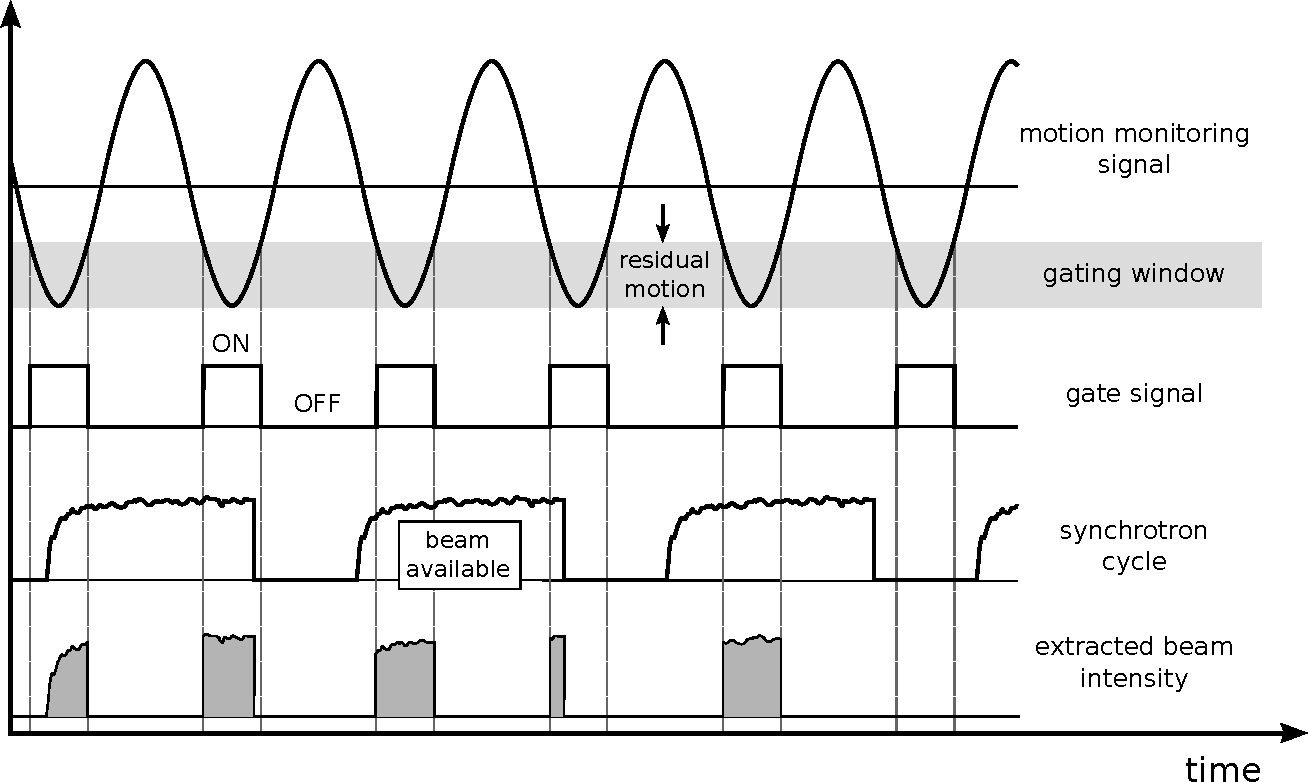
\includegraphics[width=0.9\textwidth]{gatingscheme}
  \caption[Diagram of the gating delivery mode with a synchrotron
  accelerator.]{Simplified diagram of the gating delivery mode with a
    synchrotron accelerator. The logical gate signal is generated by
    applying the \acf{GW} to the motion monitoring signal. Irradiation
    is only possible if the gate signal is active during beam
    availability. The amount of residual tumor motion depends on the
    \ac{GW} size.}
  \label{fig:background:gating}
\end{figure}
Beam gating is the irradiation in a selected part of the breathing
cycle only, the \emph{\acf{GW}}
\citep{Minohara2000,Lu2006}. Typically, the rather stable and
reproducible exhale position is chosen as the center of the \acl{GW}.
The extraction of the beam is controlled using a motion monitoring
signal (section \ref{sec:background:monitoring}). A major disadvantage
of this technique is the prolonged treatment time due to the frequent
interruptions of the beam. In figure \ref{fig:background:gating} the
principle of gating is shown schematically for a synchrotron
accelerator. As depicted, the additional folding of the gate signal
with the accelerator's duty cycle results into even longer treatment
times. However, it has been shown that optimization of the synchrotron
cycle is possible and can considerably limit the increase in treatment
time \citep{Tsunashima2008}. The efficiency can be further improved by
the extraction of multiple beam gates per synchrotron pulse
(spill). For that purpose, so-called \emph{\ac{KOE}} has been
implemented at a number of facilities, including \ac{HIT}
\citep{Noda1996,Heeg2004}.

Gating has successfully been used for the treatment of lung and liver
cancer at several centers with passive beam delivery systems
\citep{Iwata2010,Hashimoto2006}. Since the \ac{GW} has a finite size,
a corresponding residual motion inevitably remains. For beam scanning
this can result into dose inhomogeneities due to the interplay
effect. For this reason to date only few gated treatments have been
performed using beam scanning. The amount of residual motion depends
on the \ac{GW} and is typically on the order of few millimeters and
therefore comparable to the situation of abdominal compression for
liver and lung tumors. The optimization of treatment plan parameters
to mitigate residual motion effects has been proposed by
\citet{Bert2009}. This is the central research topic of this work and
will be dealt with in chapters
\ref{chap:beamopt}--\ref{chap:tpstudies}. An alternative approach
is pursued by \ac{NIRS} and \ac{PSI}, in which additional plan
robustness can be gained by combining gating with the rescanning
technique \citep{Furukawa2007,Zenklusen2010}.

%
% reference for gating at HIT?
%

\subsubsection{Rescanning/Repainting}
%\paragraph{Rescanning/Repainting}
The rescanning technique is a specific approach for scanned beam
delivery. It aims at a statistical leveling of the dose
inhomogeneities originating from beam interference effects by
performing repeated fractional irradiation of the same volume
\citep{Phillips1992}. A number of rescan options have been proposed so
far, all having their specific characteristics
\citep{Furukawa2007,Rietzel2010,Zenklusen2010}. The major discussed
options are \emph{slice-by-slice} rescanning and \emph{volumetric}
rescanning. A number of groups have proposed strategies to
additionally ensure the statistical leveling of the dose after a
number of rescans, namely \emph{random-delay rescanning}
\citep{Seco2009,Rietzel2010} and \emph{phase-controlled rescanning} or
\emph{breath-sampled rescanning}. In the latter two the rescans are
performed equally distributed over the respiratory cycle, resulting
into fewer required rescans and increased robustness.
\citep{Furukawa2010,Seco2009}.

In contrast to gating, rescanning requires to enlarge the treated
volume to at least the envelope of the tumor in all motion
states. This may result in considerable dose to normal tissue and
constitutes a major disadvantage of the technique. Despite the
breath-sampled options, the delivery of rescanning is technically
simple and does not require real-time motion monitoring
(section~\ref{sec:background:monitoring}). So far, rescanning has not
yet been established in patient treatments but is planned for the
future, \eg, at \ac{NIRS} \citep{Furukawa2007} and \ac{PSI}
\citep{Zenklusen2010}.

\subsubsection{Beam tracking}
Beam tracking was originally proposed for photon \ac{IMRT}
\citep{Keall2001}. The underlying concept is to adjust the treatment
beam with respect to the tumor and to establish the full compensation
of the target motion such that no additional margins will be
required. Beam tracking is clinically used in x-ray radiosurgery in
the robotic Cyberknife Synchrony system (Accuray Inc.\@, Sunnyvale,
Ca.\@, \acs{USA}) \citep{Brown2007a,Kilby2010}.

A full tracking system for scanned beam delivery has been implemented
at \ac{GSI}. Lateral compensation is performed with the two scanner
magnets, while longitudinal range adjustment requires fast energy
modulation via a linear motor-driven double wedge system
\citep{Weber2000}. The correction of the beam position is performed
based on a motion monitoring signal and pre-calculated look-up tables
for the compensation parameters. The system has been fully integrated
into the \ac{GSI} \acl{TCS}. Dosimetric and technical tests have
proven high precision of the system
\citep{Bert2007,Bert2010,Saito2009}. Reliable clinical use of the
system, however, requires accurate \ac{4D} imaging data and fast and
precise real-time internal motion monitoring to ensure proper
functioning of the motion compensation. This is currently not
feasible.

\subsection{Motion monitoring}
\label{sec:background:monitoring}
The application of motion monitoring in radiotherapy is manifold,
ranging from passive monitoring over interlock generation during
treatment delivery to active beam delivery control as in the beam
gating or beam tracking techniques discussed above. Motion monitoring
techniques can be grouped into those directly measuring the tumor
position, as in fluoroscopic imaging \citep{Shirato2000, Berbeco2004}
or with electromagnetic transponders \citep{Balter2005}, and motion
surrogates utilizing body surface expansion, air flow or other
secondary signals. Commercially available system, \eg, are the Varian
RPM system (Varian Medical Systems, Inc.\@) using infrared reflective
markers in combination with a camera tracking system and the \ANZAI
AZ-773V system (\ANZAI MEDICAL CO.\@, LTD) employing either laser
distance or pressure sensors attached to a waist belt
\citep{Li2006}. Surrogate motion monitoring systems do not allow for
absolute measurement of organ motion. Instead, they are used to detect 
the motion state of the patient relative to the respiratory cycle.

% amplitude, phase-based reconstruction, graph

% Evidently, the monitoring and assessment of organ motion over time is
% important. Different techniques have developed and can be divided into 
% internal and external (surrogate) motion monitoring.

% \textbf{Internal} motion monitoring techniques facilitate a
% measurement of the moving anatomy, \eg, by fluoroscopy imaging with or
% without fiducials or implanted electromagnetic transponders and
% therefore give a direct estimate of organ motion.

% \textbf{Surrogate} motion monitoring obtains indirect information of
% the patient's motion state using, \eg, optical markers, stereo camera
% systems, spirometry, pressure sensors, laser distance sensors or
% others.

% ANZAI
% what else? Corellation, use cases

\section{Treatment planning}
\label{sec:background:planning}
%
% volume definitions
%
% \begin{SCfigure}[][tbp]
%   \centering
%   \parbox[c]{0.5\textwidth}{\centering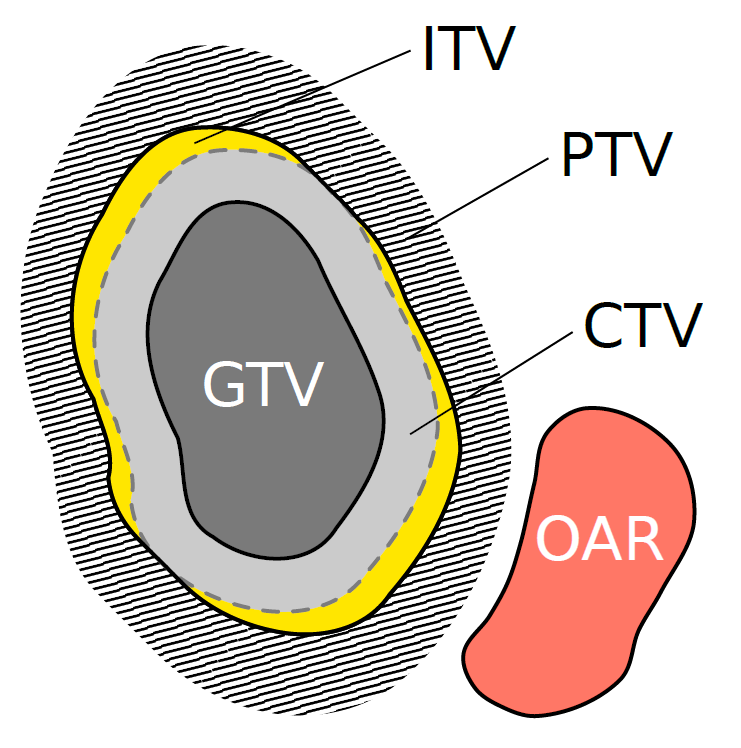
\includegraphics[width=0.35\textwidth]{volumes}}
%   \caption[Definition of volumes for treatment planning.]{Definition
%     of volumes for treatment planning. The \acf{CTV} encompasses a
%     demonstrable \acf{GTV} and/or possible microscopic spread of the
%     tumor. The \acf{PTV} takes into account geometric
%     uncertainties and avoidance of organs at risk (\acs{OAR}).}
%   \label{fig:background:volumes}
% \end{SCfigure}

% The goal of treatment planning is the definition of all machine
% parameters needed, in order to deliver a prescribed dose to a defined
% target volume while ensuring maximum possible sparing of normal
% tissue. In particular critical dose constraints for normal tissue
% complications must be respected.
Modern three-dimensional treatment planning is based on a \ac{CT} of
the volume of interest. The volumetric dataset is the basis for the
delineation of the target volume, nearby organs and critical
structures by a physician. Other fused volumetric data sets like
\ac{MRI} or \ac{PET} can be used in support during the delineation
process. The common definitions of the different treatment volumes
have been introduced in the last section (\cf
figure~\vref{fig:background:volumesitv}). The core task of treatment
planning is the dose optimization process. That is the determination
of the machine-dependent delivery parameters needed to yield the
prescribed---usually homogeneous---\ac{PTV} dose coverage for a
chosen beam configuration while minimizing the dose to normal tissue.
According to recommendations by the \ac{ICRU}, \SI{100}{\%} of the
\ac{PTV} volume should receive between \SI{95}{\%} and \SI{107}{\%} of
the planned dose \citep{ICRU50}. The dose optimization is normally
performed in an iterative computational way using a
\ac{TPS}. Treatment planning strongly depends on the employed
radiation type and the beam delivery technique. The following section
will concentrate on the specifics for scanned ion beam therapy.

\subsection{Treatment planning for scanned ion beams}
\label{sec:background:TP}
In treatment planning for scanned ion beams the characteristics of the
active beam delivery system and the physical interactions of the ion
radiation in the tissue have to be considered. For heavier ions than
protons the modeling of the biological effectiveness adds additional
complexity, due to the multiple dependencies of the \ac{RBE} (section
~\ref{sec:background:radiobiology}). Several treatment planning
systems have been developed at the different centers employing beam
scanning, \eg, at \ac{PSI} \citep{Scheib1993} and at \ac{NIRS}
\citep{Inaniwa2008}. In the following, the fundamental steps in
treatment planning with the \ac{GSI} treatment planning system,
\TRiPNE, will be briefly introduced, as they are of further interest
later in this work.  A detailed description of the program and the
underlying concepts can be found elsewhere
\citep{Kraemer2000,Kraemer2000a}.

The treatment planning process is aimed at the optimization of a
treatment plan which is applicable with the raster-scanner system
(section \ref{sec:background:activedelivery}) and yields a prescribed
(biologically effective) dose distribution. The plan consists of
raster points in a defined order (scan path). They are organized in
slices of specific energy and beam \ac{FWHM}. The optimization task is
to determine the required energies, positions and particle numbers of
all superimposed pencil beams, so that the optimal target dose
distribution is obtained.  The employed physical beam model uses a
pencil beam approach with a Gaussian beam profile in combination with
measured depth-dose curves in water. Lateral scattering is included
based on Moli\`ere's theory \citep{Moliere1948}. Ion transport model
calculations take into account nuclear fragmentation and yield
secondary particle spectra in energy and atomic number. Tissue
inhomogeneities are accounted for using the planning \ac{CT}
dataset. The \acp{HU} (representing x-ray attenuation, thus,
essentially the electron density) are voxel-wise\footnote{A voxel is
  a volume element and the \thrD analogon of a pixel.} related to a
\ac{WEPL} using a piece-wise linear calibration curve which has been
determined in dedicated measurements with tissue-equivalent materials
\citep{Geiss1999,Jaekel2001,Rietzel2007}.  Calculation of the
biological effectiveness in \TRiPNE is performed using the \acl{LEM}
(section~\ref{sec:background:radiobiology}). Starting from the
secondary particle spectra in energy and atomic number the model is
able to relate local ionization densities to a biological
effectiveness at any point in the treatment field. Dose optimization
is performed iteratively and takes into account the \ac{RBE} for each
target voxel. The algorithm initially distributes raster points
according to the requested raster spacing in each of the energy layers
covering the target in water-equivalent space. The subsequent least
square minimization algorithm determines the required particle
fluences per raster point. The physical and biological beam models are
used to calculate the dose contributions from all raster points to
each individual target voxel.

It should be noted that the modeling of the beam delivery in \TRiPNE
does not include any time structure, \ie it neglects the subsequent
nature of the beam scanning process and any target motion. The tumors
treated in the \ac{GSI} pilot project were mostly tumors of the brain
and pelvis which could be well immobilized. Thus, they were considered
static on the time-scale of the treatment delivery and no interference
with the beam scanning had to be taken into account. Per definition
this is no longer the case for intra-fractionally moving tumors. For
treatment of this kind of tumors \ac{4DTP} is essential.


\subsection{4D treatment planning}
\label{sec:background:4DTP}
It has been shown by several studies that higher tumor dose, \eg, in
lung cancer, can significantly improve local tumor control rates
\citep{Rosenzweig2005,Kong2005}. It is also observed that
radiation-induced complications depend significantly on the normal
tissue dose. For instance, Belderbos \etal report that the probability
of acute esophagus toxicity in treatment of lung cancer is
significantly correlated with the volume receiving a dose of at least
\SI{35}{Gy} \citep{Belderbos2005}. The objective of \ac{4DRT} is to
increase the dose to the moving tumor while sparing the normal tissue
and can be defined as \emph{``the explicit inclusion of the temporal
  changes in anatomy during the imaging, planning and delivery of
  radiotherapy''} \citep{Keall2004}. This section will concentrate on
the planning aspect of \ac{4DRT}. In the following, the technical
prerequisites for \acl{4DTP} will be described. Emphasis will be put
on \ac{4DTP} for ion beams. Further details on \ac{4DTP} aspects will
then follow in the subsequent chapter which focuses on the development
of a \ac{4DTPS} for ion beams.

%
% references to Chen2007, Knopf2010a and Rietzel2005a?
%

\subsubsection{Time-resolved computed tomography}
%\paragraph{Time-resolved computed tomography}
The basis for \ac{4DTP} is \emph{\ac{4DCT}} which was developed at
several centers in the past decade and is now readily available
\citep{Ford2003,Keall2004,Rietzel2005} in clinical
routine. \ac{4DCT} data acquisition is performed in dedicated
protocols which ensure that projection data of the rotating x-ray
tubes are taken over a full respiratory cycle at each couch
position. The projections are assigned retrospectively to the
respective state of motion. Time correlation between the patient
motion and the time stamp of the projections is established using
a surrogate motion monitoring device
(section~\ref{sec:background:monitoring}). The reconstruction process
yields a time series of \acp{3DCT} capturing the change of anatomy
over time. Typically, on the order of ten respiratory states are
acquired. The distribution of these so-called \emph{\ac{4DCT}
  phases}\footnote{The terms \emph{motion phase} and \emph{motion
    state} are also used frequently in the literature and will be used
  synonymously here.}  over the respiratory cycle depends on the
employed protocol. The \ac{4DCT} phases can, for instance, be defined
using the amplitude (amplitude-based), or the phase (phase-based) of
the surrogate signal \citep{Lu2006b}.

\subsubsection{Image registration and contour propagation}
%\paragraph{Image registration and contour propagation}
%
% figure registration
%  
\begin{figure}[tbp]
  \centering
  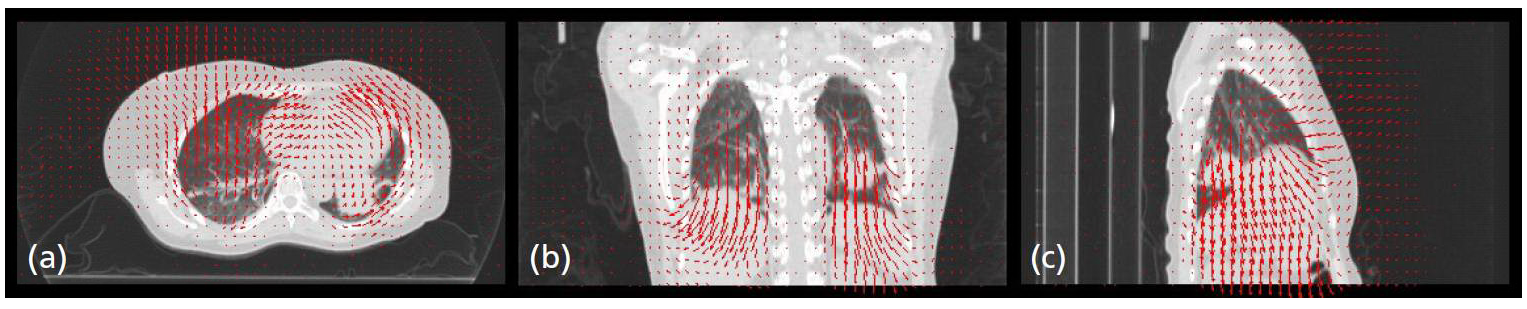
\includegraphics[width=\textwidth]{registration}
  \caption[\acl{4DCT} and image registration]{Axial (a), coronal (b)
    and sagittal (c) view of the reference \ac{4DCT} phase (end-exhale)
    of a lung cancer patient. The deformation field transforming it to
    the end-inhale phase is visualized by the overlayed vector
    field. The predominant motion in \ac{SI} direction is
    characteristic of respiration-induced motion.}
  \begin{tikzpicture}[overlay,xshift=-82mm, yshift=33mm]
    \node (a) [text=white,font=\sffamily,scale=0.9] at (0,0) {(a)};
    \node (b) [text=white,font=\sffamily,scale=0.9] at (5.8,0) {(b)};
    \node (c) [text=white,font=\sffamily,scale=0.9] at (11.55,0) {(c)};
  \end{tikzpicture}
  \label{fig:background:registration}
\end{figure}

The information provided by \ac{4DCT} on the temporal changes of the
anatomy can only be used to the full extent if a spatial correlation
between the individual \ac{4DCT} phases is established, \ie image
registration is performed. Image registration establishes a
voxel-to-voxel mapping from a reference phase to any other phase of
the breathing cycle. In figure~\ref{fig:background:registration} the
end-exhale phase of a the \ac{4DCT} of a lung cancer patient is shown,
including the deformation fields matching it with the end inhale
phase. Usually rigid registration and deformable registration methods
are distinguished. Various registration algorithms have been published
in the literature \citep{Hill2001,Brock2006,Rietzel2006a}. The
performance and accuracy of some of the available algorithms has been
evaluated recently in a dedicated multi-institutional study
\citep{Brock2010}. Brock \etal found that the registration accuracy
for the majority of the algorithms is on the order of the \ac{CT}
voxel size, \ie millimeters. However, their findings also indicate
that image registration accuracy is dependent on the image contrast.
It should be noted that registration inaccuracies translate directly
into further treatment planning steps, such as \ac{4D} image
segmentation.

Ideally, delineated structures on all \ac{4DCT} phases are available
for the subsequent steps in \ac{4DTP}. The amount of image data in
\ac{4D} imaging is increased roughly by one order of magnitude
compared to \thrD imaging. Thus, manual contouring, as in a
conventional work flow, is time-consumptive and in general not
feasible. Therefore, contour propagation methods are often used to
automate this procedure.  An overview of the available techniques can
be found in \citep{Xing2007}. One approach is to propagate the
manually contoured \ac{ROI} on the reference phase to all other phases
by using the deformation maps obtained by image registration
\citep{Lu2006a}. Alternatively, elastic deformable models can be
employed which locally adjust the reference phase contours to the test
image by physical modeling of image forces \citep{McInerney1996}.

\subsubsection{Target volume definition and motion mitigation}
%\paragraph{Target volume definition and motion mitigation}
% \ac{4D} planning strategies strongly depend on the employed delivery
% technique and radiation type. 
As already introduced in section \ref{sec:background:mitigation}, a
widely used approach to include organ motion into the planning process
is the generation of an \emph{\acf{ITV}} which is formed by the union
of the \ac{CTV} in all relevant motion phases
\citep{ICRU62}. Different options of this geometrical concept have
been reported for photon therapy
\citep{Rietzel2006b,Orban2007,Wolthaus2008}. For ion beams this
geometrical approach is not sufficient \citep{Moyers2001,ICRU78} and
needs to be modified, taking into account range variations of the
beam.  An overview of the techniques currently used for passively
delivered ion beams was published recently by Bert and Durante
\citep{Bert2011}. For scanned ion beam therapy an approach based on
\ac{4DCT} has been proposed \citep{Bert2007,Rietzel2010}. In the most
recent version the full target dimensions in water-equivalent space in
the respective motion phases are considered for the design of the
\ac{ITV}. It should be noted that the formation of the \ac{ITV}
depends on the employed motion mitigation technique. For beam gating,
for instance, \ac{ITV} generation needs to be performed using the
\ac{4DCT} phases in the \acl{GW} only.

\citet{Bert2007} have incorporated \ac{4DTP} functionality for gating,
rescanning and tracking into the \ac{GSI} \acl{TPS} \TRiPNE. Apart
from the \ac{ITV} generation for rescanning and gating, optimization
of compensation parameters for beam tracking are supported. The basic
planning strategy in TRiP98 is to optimize a treatment plan on a
reference \ac{4DCT} phase and to ensure adequate dose coverage of the
target volume in the other phases either by optimization of
compensation parameters in beam tracking or by the use of an appropriate
\ac{ITV} in combination with gating or rescanning. However, as
introduced in section~\ref{sec:background:mitigation}, the mere use of
enlarged margins, \ie an \ac{ITV}, is not sufficient for scanned
beams. Even in the case of gating or small uncompensated target
motion---as in treatments under abdominal compression---residual
motion will induce interplay effects. Bert \etal have proposed to
optimize the beam's \ac{FWHM} and the distance of \aclp{IES} to
mitigate the resulting dose inhomogeneities \citep{Bert2009}. The
research questions addressed in this dissertation are tying up to
these investigations.

\subsubsection{\acs{4D} dose calculation and optimization}
%\paragraph{ac{4D} dose calculation and optimization}
Complementary to the treatment plan optimization step \ac{4D}
dose calculation is an important tool in \ac{4DTP}. For ion beams it
allows to quantify dose heterogeneities caused by interplay
effects. \ac{4D} dose calculation algorithms exploiting deformable
image registration have been developed by several groups. Depending on
the \ac{4DCT} sampling technique, weighting of the individual dose
distributions is needed for photons and passive ion beam delivery
\citep{Rietzel2005}. For scanned beams the time-structure of the
sequential plan delivery has to be considered
\citep{Bert2007,Paganetti2004}. Summation of the individual dose
contributions is either done by transforming dose contributions in
each phase to a common reference frame \citep{Bert2007} or by
deforming the dose grid \citep{Knopf2010b}. The latter approach has
the advantage that it also enables for biological dose calculation,
which is particularly important for heavy ion therapy. Based on this
principle, Gemmel \etal have implemented a \ac{4D} dose algorithm into
the \ac{GSI} \ac{TPS} which is capable of biological and physical dose
calculations \citep{Gemmel2011}. The algorithm was validated in cell
survival measurements using a dedicated phantom. The implementation
and validation of \ac{4D} dose calculation and the modelling of
interplay effects will be dealt with in further detail in the next
chapter.

In contrast to the strategy of planning on a reference phase only, the
full incorporation of the complete \ac{4DCT} information into the dose
optimization process seems promising.  At the time of writing
no full \ac{4D} optimization has been reported for particle beams.
However, several attempts have been made for x-ray
therapy. \citet{Unkelbach2009}, \eg, have studied robust treatment plan
optimization based on probability distributions of patient
geometries. \citet{Suh2009} and \citet{Nohadani2010} have developed
robust inverse planning techniques for \ac{IMRT} motion tracking that
incorporate possible variations in the patient's breathing cycle.

\section{Summary}
In this chapter the rationale for the clinical application of ion beam
radiation has been defined and the physical and biological properties
of ions have been introduced. Their specific advantages and
characteristics have been described and the different existing
techniques to deliver ion beams to the tumor volume were discussed.
Emphasis was put on the beam scanning technique. Furthermore, the
problem of organ motion in modern radiotherapy has been illuminated
and the different existing techniques to manage organ motion effects
have been introduced. In particular, the mitigation of interplay
effects for scanned beams and of the induced changes in radiological
depth has been motivated. In the last section the requirement of
dedicated \ac{4DTP} for scanned ion beams was clarified and an
overview of the current state of research in the field was given. To
address the subject of this dissertation---the mitigation of residual
tumor motion---a functional \ac{4DTPS} is indispensable. The posed
problem required a substantial revision of the existing \ac{GSI}
\ac{4D} treatment planning functionality and its integration into a
new software. The implementation of this system will be described in
the subsequent chapter.

%%% Local Variables:
%%% TeX-master: "thesis"
%%% End:
